
\section{Model categories}

We now turn our eye to the homotopy theory of DG-algebras. Homotopy theories are described by structures called model categories. These are categories with additional structures, called model structures. Having such a model structure on a category allows us to define the notion of homotopy, which again allows us to define homotopy equivalences, and the other homotopical constructions we are used to from the homotopy theory of topological spaces. We first construct the theory abstractly, and afterwards prove that our category of interest, $DGA_k$, admits such a theory. 

\begin{definition}[Retraction]
\label{def:retraction}
\index{Retraction}
We say a map $f:A\longrightarrow B$ is a retract, or a retraction of a a map $g:X\longrightarrow Y$ if there exists a commuting diagram 
\begin{center}
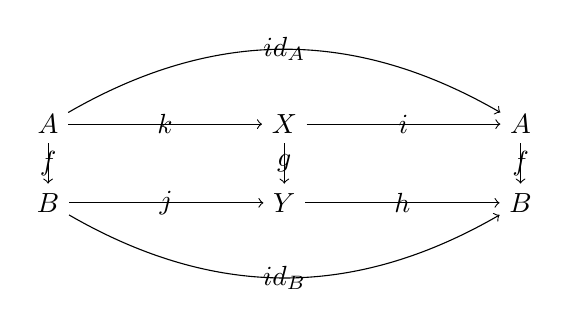
\begin{tikzpicture}
	\node (1) {$A$};
	\node (2) [below of=1] {$B$};
	\node (3) [node distance=3cm, right of=1] {$X$};
	\node (4) [below of=3] {$Y$};
	\node (5) [node distance=3cm, right of=3]{$A$};
	\node (6) [below of=5] {$B$};
	
	\draw [-to] (1) to node [swap]{$f$} (2);
	\draw [-to] (1) to node [swap]{$k$} (3);
	\draw [-to] (2) to node {$j$} (4);
	\draw [-to] (3) to node {$g$} (4);
	\draw [-to] (5) to node {$f$} (6);
	\draw [-to] (4) to node {$h$} (6);
	\draw [-to] (3) to node [swap]{$i$} (5);
	\draw [-to, bend left] (1) to node {$id_A$} (5);
	\draw [-to, bend right] (2) to node [swap] {$id_B$} (6);	
\end{tikzpicture}
\end{center}
such that the horizontal maps compose to the identity. 
\end{definition}

\begin{definition}[Retraction closed]
\label{def:retraction_closed}
\index{Retraction closed}
A class of morphisms $R$ is called retraction closed if every retraction of a morphism in $R$ is again in $R$. 
\end{definition}

Note that if a retraction closed class contains all the identitiy morphism, then it must contain all isomophims as well. 



\begin{definition}[Model structure]
\label{def:model_structure}
\index{Model structure}
Let $\mathcal{C}$ be a category. A model structure on $\mathcal{C}$ is a choice of three distinguished collections of maps, $F$, $C$ and $W$, in $\mathcal{C}$
such that the axioms below hold. The maps in the collections are called \emph{fibrations}\index{Fibration}, \emph{cofibrations}\index{Cofibration} and \emph{weak equivalences}\index{Weak equivalence} respectively, and maps in $F\cap W$ are called \emph{acyclic fibrations}\index{Acyclic fibration} and maps in $C\cap W$ are called \emph{acyclic cofibrations}\index{Acyclic cofibration}. The axioms are:

\textbf{MC1:}
Any retraction of a map in one of the three classes is again in the same class, i.e. all three classes are retraction closed. 

\textbf{MC2:}
The collection $W$ of weak equivalences has the two out of three property, i.e. if two out of $f, g, g\circ f$ is a weak equivalence, then the third is as well.

\textbf{MC3:}
If we have a commutative square 

\begin{center}
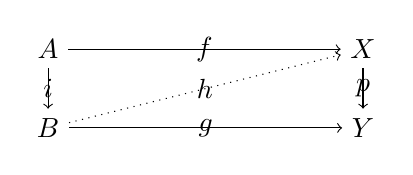
\begin{tikzpicture}
	\node (1) {$A$};
	\node (3) [below of=1] {$B$};
	\node (2) [node distance=4cm, right of=1] {$X$};
	\node (4) [below of=2] {$Y$};

	\draw [-to] (1) to node {$f$} (2);
	\draw [-to] (1) to node [swap]{$i$} (3);
	\draw [-to] (2) to node {$p$} (4);
	\draw [-to] (3) to node [swap]{$g$} (4);	
	\draw [-to, dotted] (3) to node {$h$} (2);
\end{tikzpicture}
\end{center}

where either $i\in C$ and $p\in F\cap W$, or $i\in C\cap W$ and $p\in F$, then there exists a lift $h$ making both subdiagrams commute.

\textbf{MC4:}
Given any map $f:X\longrightarrow Y$ in $\mathcal{C}$ we can factor it as $f=p\circ i$, where $p\in F$ and $i\in C\cap W$ and as $f=p'\circ i'$ where $i'\in C$ and $p'\in F\cap W$. 
\end{definition}

We then define a \emph{model category}\index{Model category} to be a bicomplete category---a category where all small limits and colimits exists---with a model structure. 

The two parts in \textbf{MC3} are often stated as fibrations having \emph{the right lifting property}\index{Right lifting property} with respect to acyclic cofibrations, and cofibrations having \emph{the left lifting property}\index{Left lifting property} with respect to acyclic fibrations. 


The archetypal example of a model category is the category of topological spaces. This category has two often used model structures, often called the Quillen (or Serre) model structure and the Strøm model structure. 

\begin{example}[Quillen model structure on topological spaces]
\label{ex:quillen_model}
The underlying category is the category of topological spaces with continuous maps. The fibrations consists of the Serre fibrations, which are maps that have the so called homotopy lifting property with respect to all CW complexes. This property is described by lifts $h$ existing when we have a CW complex $X$, and a diagram
\begin{center}
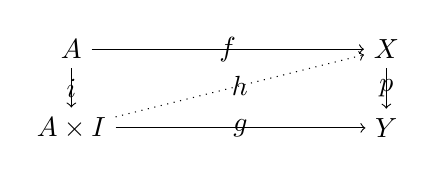
\begin{tikzpicture}
	\node (1) {$A$};
	\node (3) [below of=1] {$A\times I$};
	\node (2) [node distance=4cm, right of=1] {$X$};
	\node (4) [below of=2] {$Y$};

	\draw [-to] (1) to node {$f$} (2);
	\draw [-to] (1) to node [swap]{$i$} (3);
	\draw [-to] (2) to node {$p$} (4);
	\draw [-to] (3) to node [swap]{$g$} (4);	
	\draw [-to, dotted] (3) to node {$h$} (2);
\end{tikzpicture}
\end{center}
where $I$ is the unit interval and $i_0:A\longrightarrow A\times I$ is the inclusion into the first component. 

The cofibrations are defined by being induced by retracts of relative CW complexes, i.e. maps $g:X\longrightarrow Y$ where $Y$ is made from $X$ by attaching cells. The weak equivalences are weak homotopy equivalences, which are maps that induce isomorphisms on all homotopy groups. 
\end{example}

\begin{example}[Strøm model structure on topological spaces]
\label{ex:strom_model}
As with the previous example, the category of interest is the category of topological spaces with continuous maps. The fibrations are the Hurewicz fibrations, which satisfies the homotopy lifting property with respect to all topological spaces, not just the CW complexes as the Serre fibrations. The cofibrations are the closed Hurewicz cofibrations, which satisfy the homotopy extension property. This property is described by a lift $h$ existing when the diagram below commutes.

\begin{center}
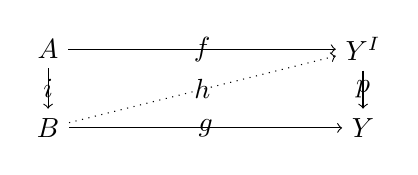
\begin{tikzpicture}
	\node (1) {$A$};
	\node (3) [below of=1] {$B$};
	\node (2) [node distance=4cm, right of=1] {$Y^I$};
	\node (4) [below of=2] {$Y$};

	\draw [-to] (1) to node {$f$} (2);
	\draw [-to] (1) to node [swap]{$i$} (3);
	\draw [-to] (2) to node {$p$} (4);
	\draw [-to] (3) to node [swap]{$g$} (4);	
	\draw [-to, dotted] (3) to node {$h$} (2);
\end{tikzpicture}
\end{center}

Here $Y^I$ is the path space of $Y$ and $p$ is the projection onto the start of a path. We call a map $i:A\longrightarrow B$ satisfying this property a Hurewicz cofibration, and we say it is a closed Hurewicz cofibration if its image is closed in $B$. The weak equivalences are given by the homotopy equivalences, i.e. the maps that are invertible up to homotopy.  
\end{example}

\begin{example}
\label{ex:cochain_complexes}
Another example is the category of positively graded cochain complexes of modules over a ring, $Ch(R-mod)$. Here the model structure consists of quasi-isomorphisms as the weak equivalences, the fibrations are degreewise projections and the cofibrations are degreewise injections with projective cokernel. The homotopy theory we get in this setting is the theory of homological algebra. 

We can expand use a similar definition for unbounded chain complexes, but then the cofibrations need a bit more care. They can however easily be defined as the morphisms that have the left lifting property with respect to the acyclic fibrations. This model category also motivates how we will define the model structure on DG-algebras, as DG-algebras are unbounded chain complexes. We can actually construct the model category of DG-algebras directly from the model category of unbounded chain complexes of vector spaces, as done in \cref{ap:A}. 
\end{example}


\subsection{Constructions in model categories}

We said that model structures allows us to introduce the notion of homotopy into the category. We will now see this construction, but first we introduce the definition of the homotopy category. Rather surprisingly, and unintuitively, this seemingly has nothing to do with homotopies at all---at least not yet. 

\begin{definition}[The homotopy category]
\label{def:homotopy_category}
\index{The homotopy category}
Let $\mathcal{C}$ be a model category and $W$ its collection of weak equivalences. We define the homotopy category of $\mathcal{C}$ to be the category $Ho\mathcal{C} = \mathcal{C}[W^{-1}]$, i.e. the localization at the weak equivalences. 
\end{definition}

\begin{remark}
The readers familiar with homological algebra will hopefully see some similarities to derived categories of rings. These are defined by localizing the category of cochain complexes of modules at the quasi-isomorphisms, which we just saw formed the weak equivalences in \cref{ex:cochain_complexes}. 
\end{remark}

Since a model category is bicomplete, it has both an \emph{initial object}\index{Initial object} $I$ and a \emph{terminal object}\index{Terminal object} $T$. Recall that these are objects where there exists a unique map from and to any other object in the category respectively. 

\begin{definition}[Fibrant object]
\label{def:fibrant}
\index{Fibrant object}
Let $X$ be an object in a model category $\mathcal{C}$. We say $X$ is fibrant if the unique map $X\longrightarrow T$ is a fibration. 
\end{definition}

\begin{definition}[Cofibrant object]
\label{def:cofibrant}
\index{Cofibrant object}
Let $X$ be an object in a model category $\mathcal{C}$. We say $X$ is cofibrant if the unique map $I\longrightarrow X$ is a cofibration. 
\end{definition}

If $X$ is both fibrant and cofibrant, we reffer to it as \emph{bifibrant}\index{Bifibrant object}. 



\begin{definition}[Cylinder object]
\label{def:cylinder_object}
\index{Cylinder object}
Let $X$ be an object in a model category $\mathcal{C}$. The cylinder object of $X$, usually denoted $Cyl(X)$, is a factorization of the codiagonal map $\nabla: X\coprod X\longrightarrow X$ into
\begin{equation*}
    X\coprod X\overset{i_0+i_1}\longrightarrow Cyl(X) \overset{p}\longrightarrow X,
\end{equation*} 
where $p$ is a weak equivalence. 

If $X\coprod X\overset{i_1 + i_2}\longrightarrow Cyl(X)$ is a cofibration, we call $Cyl(X)$ a \emph{good cylinder object}\index{Good cylinder object}, and if in addition $p$ is an acyclic fibration, we call $Cyl(X)$ a \emph{very good cylinder object}\index{Very good cylinder object}.
\end{definition}

\begin{definition}[Path object]
\label{def:path_object}
\index{Path object}
Given an object $X$ in a model category $\mathcal{C}$ we define the path object of $X$, denoted $Path(X)$ to be factorization of the diagonal map $\Delta\colon X \longrightarrow X\prod X$ into
\begin{equation*}
     X \overset{i}\longrightarrow Path(X) \overset{(p_1,p_2)}\longrightarrow X \prod X,
\end{equation*}
where $i$ is a weak equivalence. Similarly to the cylinder object, if $Path(X)\overset{p}\longrightarrow X\prod X$ is a fibration, we call $Path(X)$ a \emph{good path object}\index{Good path object}, and if in addition $i$ is an acyclic cobfiration, we call $Path(X)$ a \emph{very good path object}\index{Very good path object}.
\end{definition}

By the factorization axiom (\textbf{MC4}) every object has at least one very good cylinder object and one very good path object. It can be useful to use these in some cases, but in other cases we can actually be interested in cylinder and path objects that aren't necessarily good, or very good. For example, in the Serre model structure on topological spaces, the standard cylinder object $Cyl(X)=X\times I$ is only a good cylinder object when $X$ is a CW complex. It would sometimes be limiting to not use this standard cylinder when working with homotopies of maps between spaces that are not CW complexes, hence the reason for the weaker definition. 

Speaking of homotopies, we now have objects that resemble what we use in the category of topological spaces to define homotopies between maps. We should then be able to define them in any model category $\C$ as well. When we define homotopies in topology, we define them as maps from the cylinder $I\times X$ such that the restriction to the boundary of the cylinder gives us the two maps we are constructing a homotopy between. This is also what motivates how we define it in the general setting for model categories, but we need to be a bit more careful. For the below definitions we assume that all objects and all morphisms lie in som model category $\C$.

\begin{definition}[Left homotopy]
\label{def:left_homotopy}
\index{Left homotopy}
Given two maps $f,g: X\longrightarrow Y$ we define a left homotopy $h:f\sim_L g$ from $f$ to $g$ to be a map $h: Cyl(X)\longrightarrow Y$ such that the following diagram commutes
\begin{center}
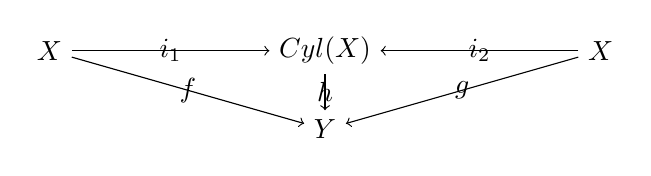
\begin{tikzpicture}
	\node (X) {$X$};
	\node (C) [node distance=3.5cm, right of=X] {$Cyl(X)$};
	\node (X') [node distance=3.5cm, right of=C] {$X$};
	\node (Y) [below of=C] {$Y$};

	\draw [-to] (X) to node {$i_1$} (C);
	\draw [-to] (X') to node [swap]{$i_2$} (C);
	\draw [-to] (X) to node [swap]{$f$} (Y);
	\draw [-to] (X') to node {$g$} (Y);
	\draw [-to] (C) to node {$h$} (Y);
\end{tikzpicture}
\end{center}
\end{definition}

\begin{definition}[Right homotopy]
\label{def:right_homotopy}
\index{Right homotopy}
Given two maps $f,g: X\longrightarrow Y$ we define a right homotopy $h:f\sim_R g$ from $f$ to $g$ to be a map $h: X\longrightarrow Path(Y)$ such that the following diagram commutes
\begin{center}
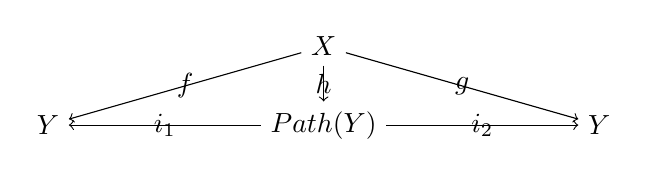
\begin{tikzpicture}
	\node (Y) {$Y$};
	\node (P) [node distance=3.5cm, right of=Y] {$Path(Y)$};
	\node (Y') [node distance=3.5cm, right of=P] {$Y$};
	\node (X) [above of=P] {$X$};

	\draw [-to] (X) to node [swap]{$f$} (Y);
	\draw [-to] (X) to node {$g$} (Y');
	\draw [-to] (X) to node {$h$} (P);
	\draw [-to] (P) to node {$i_1$} (Y);
	\draw [-to] (P) to node [swap]{$i_2$} (Y');
\end{tikzpicture}
\end{center}
\end{definition}

If the cylinder object used to define the left homotopy is a good cylinder object then we call the homotopy a \emph{good left homotopy}\index{Good left homotopy}, and similarly if it is a very good cylinder object we call the homotopy a \emph{very good left homotopy}\index{Very good left homotopy}. The same goes for the path object used to define the right homotopy, which gives us \emph{good right homotopies}\index{Good right homotopy} and \emph{very good right homotopies}\index{Very good right homotopy}.

The fact that homotopy is an equivalence relation on classes of continuous maps is one of the most important, and fundamental properties, that homotopy has in the category of topological spaces. Thus it should also be important in the general setting. Before we do that, we note that we can upgrade any left homotopy $h$ to a good left homotopy by factoring the map $X\longrightarrow Cyl(X)$ into $X\longrightarrow Cyl(X)' \overset{\sigma}\longrightarrow Cyl(X)$ by \textbf{MC4}. Then $h\circ \sigma$ will be a good homotopy. If $Y$ is fibrant, then we can upgrade it further to a very good left homotopy by using the other factorization on $Cyl(X)\longrightarrow Y$ to get $Cyl(X)\longrightarrow Cyl(X)'\longrightarrow Y$. This factorization gives us a commutative diagram
\begin{center}
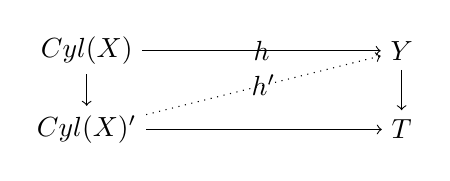
\begin{tikzpicture}
	\node (C) {$Cyl(X)$};
	\node (C') [below of=C] {$Cyl(X)'$};
	\node (Y) [node distance=4cm, right of=C] {$Y$};
	\node (T) [below of=Y] {$T$};

	\draw [-to] (C) to node {$h$} (Y);
	\draw [-to] (C) to node {} (C');
	\draw [-to] (C') to node {} (T);
	\draw [-to] (Y) to node {} (T);	
	\draw [-to, dotted] (C') to node {$h'$} (Y);
\end{tikzpicture}
\end{center}
where $T$ is the terminal object. The lift $h'$ comes from \textbf{MC3} and gives us the very good left homotopy that we wanted. 

\begin{lemma}
Let $X$ and $Y$ be objects in a model category $\mathcal{C}$. If $X$ is cofibrant then left homotopy defines an equivalence relation on $Hom(X,Y)$.
\end{lemma}
\begin{proof}
Using $X$ itself as a cylinder object together with the map $f:Cyl(X)=X\longrightarrow Y$ as a left homotopy shows that any map $f:X\longrightarrow Y$ is left homotopic to itself. It is symmetric---as we can compose with the switching map $X\coprod X \longrightarrow X\coprod X$---that just switches the components. This gives a homotopy “in the other direction”. Lastly, let $f_1\sim_L f_2$ and $f_2\sim_L f_3$ be good homotopies with cylinder objects being $Cyl(X)$ and $Cyl(X)'$ respectively. Then the pushout of the diagram $Cyl(X)' \longleftarrow X \longrightarrow Cyl(X)$ defines a new cylinder object and a homotopy $f_1\sim f_3$. Hence the relation is reflexive, symmetric and transitive which is the definition of an equivalence relation.
\end{proof}

Dually, we also get the exact same result for right homotopy, but we have to switch from $X$ being cofibrant to $Y$ being fibrant. This is because from a model structure on a category $\mathcal{C}$ we also get a model structure on its opposite category. Here the classes of fibrations and cofibrations are switched, but the weak equivalences stay the same. 

It might feel uneasing that we now have two different concepts of homotopy, which we usually don't have when working in topological spaces. There is a good reason for this, because in both the Serre and the Strøm model structure on topological spaces, all objects are fibrant. Hence, by the next lemma, the existence of right homotopies always implies the existence of left homotopies in the category of topological spaces, which means we don’t ever need to make the distinction between them.

\begin{lemma}
Let $f,g:X\longrightarrow Y$ be two maps. If $X$ is cofibrant and $f,g$ are left homotopic then they are right homotopic. Dually, if $Y$ is fibrant and $f,g$ are right homotopic, then they are left homotopic.
\end{lemma}
\begin{proof}
Choose a good cylinder object $X\coprod X \overset{i_1 + i_2}\longrightarrow Cyl(X) \overset{j}\longrightarrow X$ and let $h:Cyl(X)\longrightarrow Y$ be a left homotopy between $f$ and $g$. Choose also a good path object $Y\overset{q}\longrightarrow Path(Y) \overset{(p_1, p_2)}\longrightarrow Y\prod Y$. We then have a commutative diagram
\begin{center}
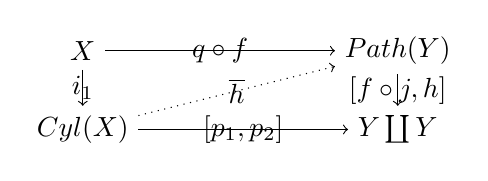
\begin{tikzpicture}
	\node (X) {$X$};
	\node (C) [below of=X] {$Cyl(X)$};
	\node (P) [node distance=4cm, right of=X] {$Path(Y)$};
	\node (Y) [below of=P] {$Y\coprod Y$};

	\draw [-to] (X) to node {$q\circ f$} (P);
	\draw [-to] (X) to node [swap]{$i_1$} (C);
	\draw [-to] (C) to node [swap]{$[p_1, p_2]$} (Y);
	\draw [-to] (P) to node {$[f\circ j, h]$} (Y);	
	\draw [-to, dotted] (C) to node {$\overline{h}$} (P);
\end{tikzpicture}
\end{center}
which has a lift $\overline{h}$ by \textbf{MC3}. 
%Note here that we used the fact that $i_1$ is an acyclic cofibration which we have not proved, but it can be seen by the two out of three property since $X$ is assumed to be cofibrant together with the fact that it is a composition of two cofibrations. 
The composition $h\circ i_2:X\longrightarrow Path(X)$ gives a right homotopy between $f$ and $g$ as desired. The dual statement is proved dually.
\end{proof}

We can then finally define the notion of homotopy as follows. 

\begin{definition}[Homtopic maps]
\label{def:homotopic_maps}
\index{Homotopic maps}
We say two maps $f,g:X\longrightarrow Y$ are homotopic, denoted $f\sim g$, if they are both left homotopic and right homotopic.
\end{definition}

This means we can finally define homotopy equivalences. 

\begin{definition}[Homotopy equivalence]
\label{def:homotopy_equivalence}
\index{Homotopy equivalence}
We say a morphism $f\colon X\longrightarrow Y$ is a homotopy equivalence if there exists a morphism $g\colon Y\longrightarrow Y$ such that $f\circ g \sim id_Y$ and $g\circ f \sim id_X$. If there exists a homotopy equivalence between two objects, we call them homotopy equivalent.
\end{definition}

If we now restrict our attention to just the bifibrant\index{Bifibrant object} objects in a model category, we see that we have a well defined notion of homotopy. It is well defined in the sense that it is an equivalence relation. A question we could ask is: when are two objects are homotopy equivalent? and how does this notion of homotopy equivalence relate to weak equivalences? We have a very nice correspondence in this setting, i.e. when restricting to the bifibrant objects. 

\begin{theorem}[Generalized Whiteheads theorem]
\label{thm:whitehead}
\index{Generalized Whiteheads theorem}
Two bifibrant objects $X$ and $Y$, in a model category $\C$, are homotopy equivalent if and only if they are weakly equivalent. 
\end{theorem}

We won't cover the proof, but refer to \cite[Theorem 1.2.10.]{hovey}. 

This means that localizing at the weak equivalences also turns homotopy equivalences of bifibrant objects into isomorphisms. If we take the subcategory of bifibrant objects, which we denote $\C_{cf}$, we can form its quotient by the homotopy relation, $\C_{cf}\longrightarrow \C_{cf}/\sim$. By the generalized Whitehead theorem this map sends weak equivalences to isomorphisms, and hence it has to factor through its homotopy category, $Ho(\C_{cf})$, by general theory about localization. We also have an inclusion $\C_{cf} \longrightarrow \C$ which induces a map on their homotopy categories, $Ho(\C_{cf})\longrightarrow Ho(\C)$. The final piece of the puzzle of having a workable homotopy category, comes from the fact that those maps form an equivalence of categories $Ho(\C)\cong \C_{cf}/\sim$, which means that we have a nice definition, and a nice way to work with it.











